% PACKAGES INCLUDED HERE 
% DO NOT NEED TO CHANGE
\documentclass[conference]{IEEEtran}
%\IEEEoverridecommandlockouts
% The preceding line is only needed to identify funding in the first footnote. If that is unneeded, please comment it out.
\usepackage{cite}
\usepackage{amsmath,amssymb,amsfonts}
\usepackage{algorithmic}
\usepackage{graphicx}
\usepackage{subcaption}
\usepackage{textcomp}
\def\BibTeX{{\rm B\kern-.05em{\sc i\kern-.025em b}\kern-.08em
    T\kern-.1667em\lower.7ex\hbox{E}\kern-.125emX}}
\begin{document}


% TITLE

\title{A Comparison of Altered Convolutional Filter Prevalence for U-Net in MRI Brain Tumor Segmentation\\}

% AUTHORs

\author{\IEEEauthorblockN{1\textsuperscript{st} Brian Sharber}
\IEEEauthorblockA{\textit{Department of Computer Science} \\
\textit{Middle Tennessee State University}\\
Murfreesboro, Tennessee USA \\
bws2u@mtmail.mtsu.edu}
\and
\IEEEauthorblockN{2\textsuperscript{nd} Lucas Remedios}
\IEEEauthorblockA{\textit{Department of Computer Science} \\
\textit{Middle Tennessee State University}\\
Murfreesboro, Tennessee USA \\
lwr2k@mtmail.mtsu.edu}
\and
\IEEEauthorblockN{3\textsuperscript{rd} Christine Monchecourt}
\IEEEauthorblockA{\textit{Department of Computer Science} \\
\textit{Middle Tennessee State University}\\
Murfreesboro, Tennessee USA \\
cfm3a@mtmail.mtsu.edu}
\and
\IEEEauthorblockN{4\textsuperscript{th} David Woods}
\IEEEauthorblockA{\textit{Department of Computer Science} \\
\textit{Middle Tennessee State University}\\
Murfreesboro, Tennessee USA \\
dmw6c@mtmail.mtsu.edu}
\and
\IEEEauthorblockN{5\textsuperscript{th} Joshua Ortner}
\IEEEauthorblockA{\textit{Department of Computer Science} \\
\textit{Middle Tennessee State University}\\
Murfreesboro, Tennessee USA \\
jo3f@mtmail.mtsu.edu}
\and
\IEEEauthorblockN{6\textsuperscript{th} Joshua LaFever}
\IEEEauthorblockA{\textit{Department of Computer Science} \\
\textit{Middle Tennessee State University}\\
Murfreesboro, Tennessee USA \\
jrl5z@mtmail.mtsu.edu}
}

\maketitle

% ABSTRACT 

\begin{abstract}
The U-Net neural network architecture is commonly used to segment brain tumors. Reducing the number of convolutional filters in U-Net would be beneficial for those with limited computational resources, as using more filters requires more VRAM. To see how performance varies with filter prevalence, we tested U-Net in 4 different experiments where we divided the number of convolutional filters in each layer by 1, 2, 4, and 8 respectively. The resulting data showed that performance was best with all the filters, but that less filters could still perform well as long as a model had a good weight initialization. Repeating the experiments with more weight initializations and longer training would be beneficial.

\end{abstract}

% KEYWORDS

\begin{IEEEkeywords}
Neural Networks, Convolutional Neural Networks, CNN, Python, Keras
\end{IEEEkeywords}

% INTRODUCTION SECTION
\section{Introduction \& Background}

% IMAGE SEGMENTATION SUBSECTION
\subsection{Image Segmentation}
The goal of image segmentation is to determine which portion of an image contains a desired feature. An image segmentation model produces a predicted mask, which shows where the feature is predicted to reside in an image. Evaluating an image segmentation model can be done in a couple of different ways. One such way is using the Dice Coefficient, which can be modified to be utilized as a loss function during training. The Dice Coefficient formula can be explained as: 2 * the Area of Overlap divided by the total number of pixels in both the input and predicted images. This is similar to the formula for IoU (Intersection over Union) which can be explained as: the number of pixels common between the input and predicted masks divided by the total number of pixels present across both masks. A Dice Coefficient of 1 indicates perfect segmentation, whereas a Dice Cofficient of 0 indicates a complete failure of  segmentation.

% CAD SUBSECTION
\subsection{CAD - Computer-Aided Diagnosis}
In the medical imaging field, CAD (computer-aided diagnosis) is a computer-based system that assists doctors with interpretation of medical images ~\cite{doi2007computer}. Imaging techniques like MRI, X-ray, endoscopy, and ultrasound yield a lot of information that a radiologist or medical professional must evaluate and understand comprehensively in a short period of time. CAD systems process medical images for the appearance of abnormalities and diseases, and highlight conspicuous sections to offer support on a medical professional’s decision for a patient~\cite{doi2007computer}.

\begin{figure}[htpb]
    \centering
    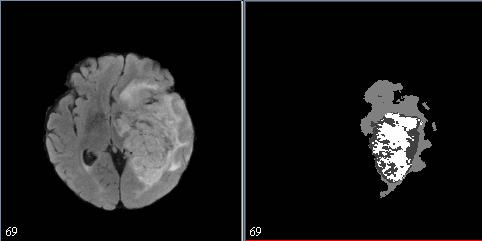
\includegraphics[width=\textwidth,height=3cm,keepaspectratio=true]{Screenshot (7).png}
    \caption{
        Sample Input Slice and Mask from the BraTS dataset ~\cite{menze2014multimodal} ~\cite{bakas2017advancing} ~\cite{bakas2018identifying} 
    }
\end{figure}

% Neural Networks SUBSECTION
\subsection{Neural Networks}
Neural networks are information processing mechanisms inspired by the operation of biological nervous systems. Convolutional neural networks (CNNs) are specialized neural networks that are commonly applied to analyzing images. U-Net is a popular CNN used for medical image segmentation ~\cite{ronneberger2015u}. 


% GPU SUBSECTION
\subsection{U-Net with GPUs}
One of the most noticeable drawbacks of a CNN, and by extension U-Net, is extensive training times. Training a CNN is computationally heavy and data-intensive. Though, larger data sets can provide a more accurate CNN, large data sets can require training to take days or even weeks. The training steps require low data transfer but a massive amount of floating point operations on that data. These characteristics make GPUs (Graphic Processing Units) ideal for the task ~\cite{strigl2010performance}.

Previously, using GPUs for general purpose calculations would require extensive knowledge of the hardware architecture. This forced algorithms to be formatted to be graphics friendly. The introduction of CUDA (Compute Unified Device Architecture) provided a much more familiar language for programmers to work in than previously used graphics APIs. However, a drawback of CUDA is that it is only applicable to Nvidia hardware ~\cite{strigl2010performance}.

GPUs are useful for training U-Net, however they pose some limitations on the network itself. GPU hardware has a limited amount of VRAM, and GPUs with more VRAM typically cost more. This causes GPU VRAM to be considered in the construction of the network. U-Net makes use of several convolutional layers within the network. The hidden units in a convolutional layer are comprised of filters that slide across the image and down-sample the input image. Even though the hidden units produce a smaller output than the input, each unit in the layer produces an output, increasing the depth of the total output for the layer ~\cite{michelucci2019advanced}. 

 As the U-Net architecture uses several convolutional layers it must be built with resources in mind to avoid over allocation of memory which would crash the program. A simple way to adjust the amount of required resources is to adjust the number of filters each convolutional layer employs.


% Project Goal
\subsection{Project Goal}
In this work, to see if we could successfully perform tumor segmentation while using less GPU RAM, we explored the effect of variably reducing the number of filters in each convolutional layer in U-Net. 


% METHODS SECTION
\section{Methods}

% Data set
\subsection{Data}

The data used in this project is from the 2019 Multimodal Brain Tumor Segmentation Challenge~\cite{menze2014multimodal}~\cite{bakas2017advancing}~\cite{bakas2018identifying}, also known as BraTS. The dataset consists of multimodal brain MRI scans. There are four different image modalities per patient: 
\par - T1: T1 refers to one of the two tissue relaxation times (longitudinal relaxation time). This modality is produced by sending short radio frequency pulses through tissue to create an image. The brightness of the image is determined mainly by the T1 properties of tissue.
\par - T1ce (post-contrast T1-weighted): This modality is a modified version of T1 described above.
\par - T2: T2 refers to the other tissue relaxation time (transverse relaxation time). This modality is created by using longer radio frequency pulses.
\par - FLAIR (T2 Fluid Attenuated Inversion Recovery volumes): This modality is created by using radio frequency pulses that are even longer than the T1 and T2 modalities. This creates an image whose abnormalities are bright, while the normal CSF fluid is dark. 
\par Along with these 4 modalities, there is also a segmentation volume (ground truth) showing where the tumor exists for each patient.

% Unet
\subsection{U-Net}
U-Net, inspired from traditional convolutional neural networks, was first designed to process biomedical images in 2015 ~\cite{ronneberger2015u}. Whereas many convolutional neural network architectures focus on image classification, U-Net was designed for solving the biomedical imaging problem of not only distinguishing whether the patient has a disease, but also localizing the area of abnormality. 

\par The U-Net architecture is symmetric, consisting of two major parts: the left part (contracting path), which is constituted by the general convolutional process, and the right part (expansive path), which can be thought of as an up-sampling technique and constituted by transposed 2-D convolutional layers. \par The contracting path consists of this formula: convolutional\_layer1 to convolutional\_layer2 to max\_pooling to dropout(optional). Each process consists of two convolutional layers; the number of channels changes from 1 to 64 as the depth of the image is increased by the convolution process. The max pooling process halves image size. The process is repeated three times; two convolutional layers are built with no max pooling.\par The expansive path consists of this formula: convolutional\_2d\_transpose to concatenate to convolutional\_layer1 to convolutional\_layer2. In this path, the image will be upsized to original size. After the transposed convolution, an up-sampling technique that expands image size takes place, the image is upsized and concatenated with the corresponding image from the contracting path. This is to combine the information from the previous layers to get a more precise prediction. \par Reaching the last layers in the architecture, the last step is to reshape the image to satisfy the prediction requirements. This entire process makes a strong enough network able to do good prediction even if your data set is small, utilizing excessive data augmentation techniques.

% Framework
\subsection{Programming Framework}
Our code was implemented using the TensorFlow ~\cite{tensorflow2015-whitepaper} and Keras ~\cite{chollet2015keras} libraries for the Python programming language.

% Data Preprocessing
\subsection{Thresholding the Masks}
To binarize the masks, all of the pixel intensities greater than 0.5 were set to 1 and all the rest were set to 0.

\subsection{Normalization}
%explain normalization
The values of the pixel intensities in this data set vary widely in magnitude, thus it was important to normalize the data to limit the range of possible values that may bias the network. The images were normalized by patient and modality. For every modality image volume, we found its max pixel intensity and divided all of its the pixel intensities by that max value. This ensured that the range of all values was between 0 and 1 and the images were scaled based on the entire modality.

\subsection{Outlier Detection}
%explain how outliers were selected
In order to eliminate a source of possible noise, it was necessary to examine the data set for potential outliers. Outliers, in this case, could include images that had portions missing, or anomalies causing an image to look different from the rest. To locate outliers, we used the MIPAV (Medical Image Processing, Analysis, and Visualization) application~\cite{mcauliffe2009medical}. Using this application, we were able to visualize the different modalities for each patient. We used this functionality to inspect each patient’s scans for abnormalities. The handful of visually identified potential outliers were removed from the data set.


\subsection{Experiment Design}
% How experiments are set up
To test how reducing the number of filters in each convolutional layer in the U-Net affects performance we ran 4 experiments. The experiments are titled DS 1 (full U-Net), DS 2 (U-Net with half the number of filters in each convolutional layer), DS 4 (U-Net with a quarter of the number of filters in each convolutional layer), and DS 8 (U-Net with an eighth of the filters in each convolutional layer). The experiments only varied by the number of filters.

Each experiment consisted of 5 runs with different neural network initializations. These 5 initializations were trained to determine how altering the number of convolutional filters affects U-Net's performance on average for our task. We used 60\% of the data for training, 20\% for validation, and 20\% for testing.

\subsection{Metrics}
%description of loss etc.
We used the dice coefficient as a way of measuring the performance of the model. A dice coefficient of 1 represents a perfect segmentation, and a dice coefficient of 0 represents a completely failed segmentation. We used dice loss as our loss function, which is 1 - the dice coefficient. Dice loss is bounded between 0 and 1.

\subsection{Training Protocol}
% The training approach
For each run (model initialization), a chunk of data of 5 patients was loaded into RAM at a time. The data for each patient consisted of 4 image volumes in 4 different MRI modalities (T1, T1CE, T2, FLAIR). These 4 image volumes were combined into a multimodal image tensor for each patient. The corresponding 5 patients’ multimodal image tensors were then stacked and shuffled slice-wise, where each slice is a multimodal slice. 20\% of each chunk was used as validation data. 

Our U-Net models take multimodal image tensor slices as input. We used a batch size of 32 for each chunk of patient data. We had 39 chunks of data per epoch, and trained each initialized model for 20 epochs.

\subsection{Testing Protocol}
%how we tested
We tested each initialized model by finding the performance on test patients’ multimodal image tensors. Each patient’s multimodal image tensor was read in, and the model made a prediction for each slice sequentially in the input tensor. For each patient, we stacked all of the predicted masks into a volume and computed a single dice coefficient volume-wise against the corresponding mask volume. 

\subsection{Dice Coefficient Differences between Training and Testing}
It is important to note, that during training, the dice coefficients were generated based on non-thresholded predicted masks, with continuous values between 0 and 1. During testing, the dice coefficients were produced on thresholded predicted masks, consisting only of binary values, 0 or 1.

% RESULTS SECTION
\section{Results}

% How numbers are computed
\subsection{Computations for Training Metrics}

Each experiment's losses (Fig. 2) and dice coefficients (Fig. 3) are computed for each epoch by finding the mean of the selected metric for each of the 5 initializations. On an initialization, the loss and dice coefficient for each epoch was computed as the average loss and dice coefficient for the 39 chunks in the epoch.

\subsection{Computations for Testing Metrics}

Each experiment's average dice coefficient was visualized by plotting the mean dice coefficient for each initialization (Fig. 4). Each initializations' dice coefficient was computed as the mean of the dice coefficient for each patient in the testing data set.   

\subsection{Training Results}
During training, the experiments performed on average in this order, ranked best to worst: DS 1, DS 8, DS 2, DS 4. It is clear that none of the 5 initializations for DS 4 learned. DS 1 had 1 very good initialization. The end-of-training average loss for each experiment is as follows: DS 1 $\xrightarrow{}$ $\sim$0.3, DS 2 $\xrightarrow{}$ $\sim$0.7, DS 4 $\xrightarrow{}$ $\sim$1, DS 8 $\xrightarrow{}$ $\sim$0.5 (Fig~\ref{fig:training_loss}). The end-of-training average dice coefficient for each experiment is as follows: DS 1 $\xrightarrow{}$ $\sim$0.75, DS 2 $\xrightarrow{}$ $\sim$0.3, DS 4 $\xrightarrow{}$ $\sim$0, DS 8 $\xrightarrow{}$ $\sim$0.5 (Fig~\ref{fig:training_dice}). 



\subsection{Testing Results}
The ordering of performance on the testing data, ranked best to worst, is the same as that of the training performance:  DS 1, DS 8, DS 2, DS 4 (Fig~\ref{fig:testing_dice}). The average dice coefficients for each experiment are as follows: DS 1 $\xrightarrow{}$ $\sim$0.9, DS 2 $\xrightarrow{}$ $\sim$0.5, DS 4 $\xrightarrow{}$ $\sim$0.3, DS 8 $\xrightarrow{}$ $\sim$0.75 (Fig~\ref{fig:testing_dice}). 


    
%training loss plot for each experiment
\begin{figure}
\centering
\begin{tabular}{cccc}
\subfloat{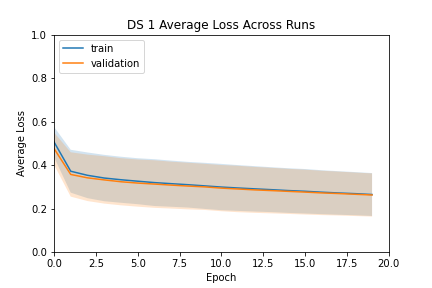
\includegraphics[width = 0.8\linewidth]{ds_1_loss_plot.png}} \\
\subfloat{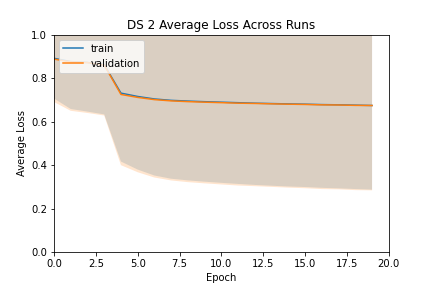
\includegraphics[width = 0.8\linewidth]{ds_2_loss_plot.png}} \\
\subfloat{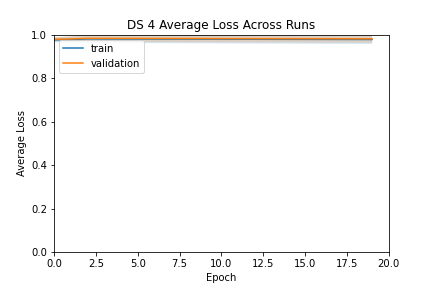
\includegraphics[width = 0.8\linewidth]{ds_4_loss_plot.png}} \\
\subfloat{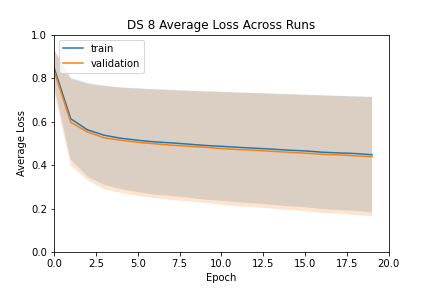
\includegraphics[width = 0.8\linewidth]{ds_8_loss_plot.png}}
\end{tabular}
\caption{Average training losses for each experiment.}
\label{fig:training_loss}
\end{figure}

%training dice plot for each experiment
\begin{figure}
\centering
\begin{tabular}{cc}
\subfloat{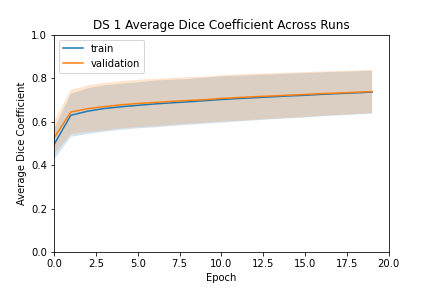
\includegraphics[width = 0.8\linewidth]{ds_1_Dice Coefficient_plot.png}} \\
\subfloat{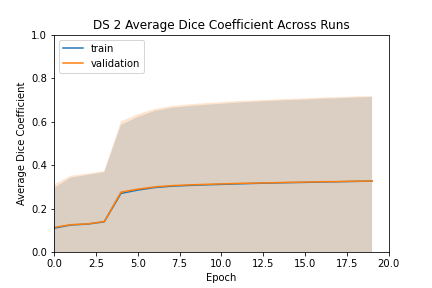
\includegraphics[width = 0.8\linewidth]{ds_2_Dice Coefficient_plot.png}} \\
\subfloat{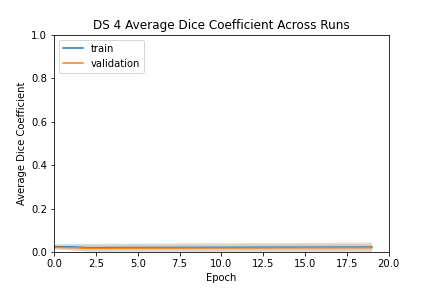
\includegraphics[width = 0.8\linewidth]{ds_4_Dice Coefficient_plot.png}} \\
\subfloat{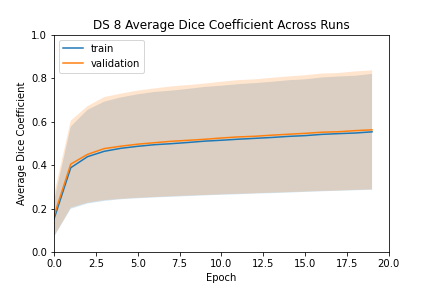
\includegraphics[width = 0.8\linewidth]{ds_8_Dice Coefficient_plot.png}}
\end{tabular}
\caption{Average training dice coefficients for each experiment.  }
\label{fig:training_dice}
\end{figure}

%testing dice plot for each experiment
\begin{figure}
\centering
\begin{tabular}{cc}
\subfloat{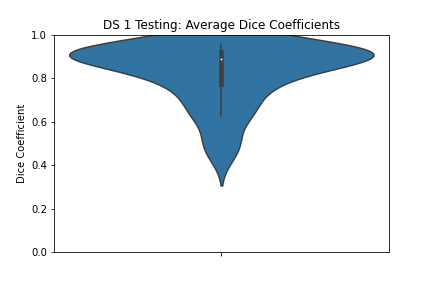
\includegraphics[width = 0.8\linewidth]{ds_1_testing_violin_plot.png}} \\
\subfloat{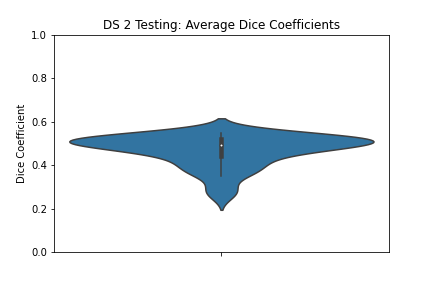
\includegraphics[width = 0.8\linewidth]{ds_2_testing_violin_plot.png}} \\
\subfloat{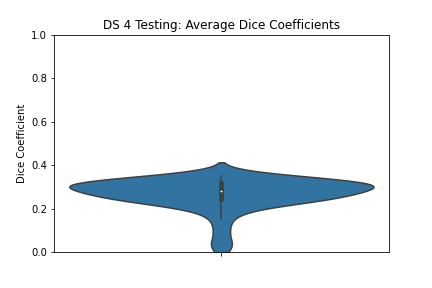
\includegraphics[width = 0.8\linewidth]{ds_4_testing_violin_plot.png}} \\
\subfloat{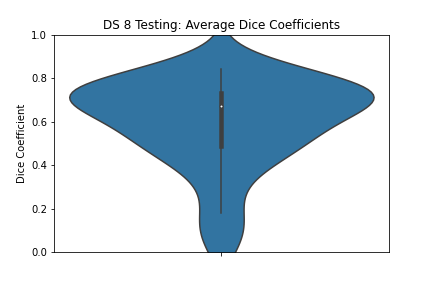
\includegraphics[width = 0.8\linewidth]{ds_8_testing_violin_plot.png}}
\end{tabular}
\caption{ Average testing dice coefficients for each experiment. }
\label{fig:testing_dice}
\end{figure}

% DISCUSSION SECTION
\section{Discussion \& Conclusion}

Looking at the average dice coefficients for the testing performed on each experiment, we can determine how well each experiment performed (Fig~\ref{fig:testing_dice}). DS 1 had the best performance, which was expected, as it had the most filters compared to the other experiments. DS 8 performed second best, which is counter-intuitive, as it had an eighth of the filters as DS 1. The expected behavior would have been for the best to worst experiment ordering to have been: DS 1, DS 2, DS 4, DS 8. 

DS 1 consistently had good initializations which enabled each run to learn the segmentation function. This was not the case for DS 4. This may expose how having less filters impacts the importance of having a good initialization, however more runs would be needed to verify this. 

None of the experiments that succeeded appear to have plateaued in performance. This indicates that training the models in each experiment longer could have produced better model performance.

These results show that U-Net with less filters can still learn tumor segmentation. To see how well less filters truly compare to more filters, future work could include training the models in each experiment longer to see if a larger model, say DS 1, and a smaller model, say DS 8 perform similarly after plateauing in performance. Additionally, more runs should be performed for each experiment to get a better average sense of how the filters affect model performance, as it seems that having only 5 runs may not be enough data to get a true reading of how filter prevalence impacts U-Net performance.

% REFERENCES
% THIS CAN BE CREATED AUTOMATICALLY
\bibliographystyle{IEEEtran}
\bibliography{refs.bib} % change if another name is used for References file




\end{document}